%1578
\newpage
\subsection{例題4-7 自分で用意した絵を動かして表示する}


\begin{description}
    \item \textgt{\bf \ \ 考え方}
\end{description}



apple.hspのプログラムを使って、自分で作った絵を動かすようにしてみましょう。

表示させるための画像は、GIMPツールで作ったり、確認することができます。GIMPは、Raspberry
Piメニューからグラフィックス→「GNU Image Manipulation Program」をクリックすることで起動させることができます。

りんごの画像は、「apple.png」です。

開くメニューから、「apple.png」を読み込んで編集してください。

背景にあたる部分は、消しゴムで消す必要があるので注意してください。


\begin{figure}[H]
    \begin{center}
      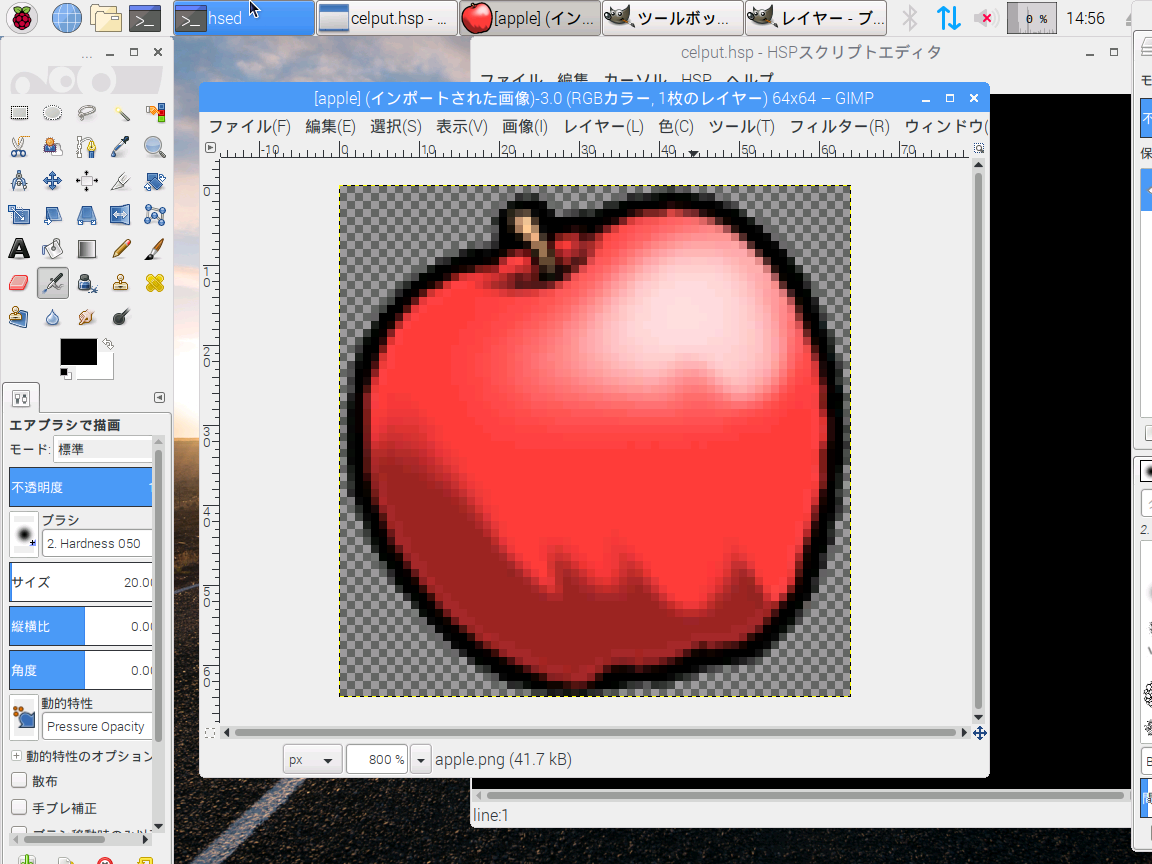
\includegraphics[keepaspectratio,width=11.712cm,height=8.784cm]{text04-img/text04-img021.png}
      \caption{GIMPの編集画面}
    \end{center}
    \label{fig:prog_menu}
\end{figure}

% \bfseries  "\ \"
\begin{description}
    \item \textgt{\bf 例題4-7 答え}
\end{description}



GIMPで修正できたら、[F5]キーを押して改造した人がきちんと表示されるかどうか確認しましょう。

自分で別な画像ファイルを用意した場合は、

\begin{description}
    \item \textgt{\bf \ \ celload “apple.png”,2}
\end{description}


のファイル名を修正してください。

元のりんご画像に戻したい時は、元のファイル(apple.png)をもう一度コピーして使ってみてください。

% Jump Action:

%1644



